\documentclass[11pt]{article}

\usepackage[T1]{fontenc}
\usepackage[utf8]{inputenc}
\usepackage[margin=1in]{geometry}
\usepackage{amsmath}
\usepackage{amssymb}
\usepackage{booktabs}
\usepackage{tabularx}
\usepackage{array}
\usepackage{xcolor}
\usepackage{listings}
\usepackage{tikz}
\usepackage[hidelinks]{hyperref}

% Inline code shorthand: monospaced, but with line-break opportunities after
% underscores so long identifiers/paths don't overflow the text block.
\newcommand{\code}[1]{\texttt{\def\_{\textunderscore\allowbreak}#1}}

% Let TeX stretch the last line a little rather than overflowing the margin.
\setlength{\emergencystretch}{3em}

\lstset{
  basicstyle=\ttfamily\small,
  breaklines=true,
  frame=single,
  framesep=4pt,
  language=Python,
  keywordstyle=\color{blue!60!black},
  commentstyle=\color{gray},
  stringstyle=\color{green!40!black},
  showstringspaces=false,
  columns=fullflexible,
}

% Plain (non-language) listing style for the ASCII flow diagram
\lstdefinestyle{plain}{language={},keywordstyle=\ttfamily,basicstyle=\ttfamily\footnotesize,breaklines=false}

\title{Propagation of energy units through pymatgen's
\texttt{HeisenbergMapper}}
\author{Luca Frey}
\date{\today}

\begin{document}
\maketitle

\begin{abstract}
\noindent
We document the propagation of energy, and of its physical units, through the
exchange-coupling fitting procedure implemented in pymatgen's
\code{HeisenbergMapper} class. Starting from the public interface of the
class---a set of magnetic structures together with their total DFT
energies---we follow the energy through normalisation, construction of the
Heisenberg design matrix, solution of the resulting linear system, and
serialisation into the \code{HeisenbergModel} object. We establish that the
only normalisation applied within the mapper is division by the number of
magnetic ions, so that the internal energy unit is electron\-volts per magnetic
ion and the fitted couplings are reported in milli\-electron\-volts per magnetic
ion, in contrast to the ``meV/atom'' label used in the source. We further derive
the condition under which the fitted couplings coincide with the physical
exchange constants, namely that every magnetic ordering entering the fit share a
common supercell size.
\end{abstract}

\section{Introduction}

This note traces the energy---and its units---from the point at which structures
and total energies are passed to pymatgen's \code{HeisenbergMapper}, through the
construction of the Heisenberg design matrix and the linear fit, to the
\code{HeisenbergModel} object that is written out. The upstream processing
(extraction of structures and energies from the magnetic-orderings document and
reconstruction of total energies) is omitted by design: the analysis begins at
the public contract of the class, that is, it assumes that the following are
already available:

\begin{itemize}
  \item a list of magnetic structures, each carrying a \code{magmom} site
        property, and
  \item a list of total energies $E_k^{\mathrm{tot}}$ (eV), each being the energy
        of the entire supercell of ordering $k$, summed over all of its atoms.
\end{itemize}

\noindent
All file and line references are to
\code{.venv/\allowbreak lib/\allowbreak python3.12/\allowbreak site-packages/\allowbreak pymatgen/\allowbreak analysis/\allowbreak magnetism/\allowbreak heisenberg.py}.

\section{Notation and energy model}

The symbols used throughout are fixed in Table~\ref{tab:notation}.

\begin{table}[h]
\centering
\caption{Notation used throughout this note.}
\label{tab:notation}
\begin{tabularx}{\textwidth}{@{}l X l@{}}
\toprule
Symbol & Meaning & Unit \\
\midrule
$E_k^{\mathrm{tot}}$ & total DFT energy of ordering $k$ (whole supercell) & eV \\
$N_k^{\mathrm{mag}}$ & number of magnetic ions in ordering $k$ & --- (count) \\
$\varepsilon_k$ & per-mag-ion energy, $\varepsilon_k = E_k^{\mathrm{tot}}/N_k^{\mathrm{mag}}$ & eV / mag ion \\
$s_i$ & local magnetic moment (\code{magmom}) on magnetic ion $i$, used as a bare number & value in $\mu_B$ \\
$J_{ab}$ & exchange constant for neighbour class $ab$ (nn/nnn/nnnn) & see Sec.~\ref{sec:fit} \\
$E_0$ & spin-independent (nonmagnetic) reference energy & eV / mag ion \\
\bottomrule
\end{tabularx}
\end{table}

\noindent
The Heisenberg energy model assumed by the code is collinear, with the moments
entering as dimensionless scalars (their bare values in $\mu_B$), so that the
energy units are carried entirely by $J$:
\begin{equation}
E^{\mathrm{tot}} = E_0 - \sum_{\langle i,j\rangle} J_{ij}\, s_i\, s_j ,
\label{eq:model}
\end{equation}
where the sum runs over unique neighbour bonds $\langle i,j\rangle$.

\paragraph{Normalisation convention.}
At no point in this pipeline is the energy normalised by the total atom count.
The only normalisation that occurs is division by the number of magnetic ions,
$N_k^{\mathrm{mag}}$. Consequently the internal energy unit of the mapper is
eV per magnetic ion, and the fitted couplings emerge per magnetic ion---not per
total atom---notwithstanding the ``meV/atom'' description used in the source
docstrings.

\section{Energy ingestion and normalisation}
\label{sec:ingestion}

The constructor \code{HeisenbergMapper.\_\_init\_\_} routes its inputs through the
helper class \code{HeisenbergScreener}, whose \code{\_do\_cleanup} method performs
the unit-relevant operations (\code{heisenberg.py:696}). Three steps are carried
out.

\begin{enumerate}
  \item \emph{Restriction to the magnetic sublattice}
        (\code{heisenberg.py:717--722}). Each structure is reduced to its
        magnetic ions via \code{get\_structure\_with\_only\_magnetic\_atoms}.
        Thereafter \code{len(s)} equals $N_k^{\mathrm{mag}}$, the magnetic-ion
        count, rather than the total atom count.

  \item \emph{Normalisation of the energy} (\code{heisenberg.py:725}):
\begin{lstlisting}
energies = [e / len(s) for (e, s) in zip(energies, ordered_structures)]
\end{lstlisting}
        This is the single, decisive unit conversion of the pipeline:
        \begin{equation}
          \varepsilon_k = \frac{E_k^{\mathrm{tot}}}{N_k^{\mathrm{mag}}}
          \qquad [\text{eV}] \;\longrightarrow\; [\text{eV} / \text{mag ion}] .
        \end{equation}
        From this point onward, every energy handled by the mapper is expressed
        in eV per magnetic ion.

  \item \emph{De-duplication and ordering} (\code{heisenberg.py:732--754}).
        Degenerate orderings are removed using a tolerance of $10^{-6}$
        eV per magnetic ion, after which the structures and energies are sorted in
        ascending order of $\varepsilon_k$.
\end{enumerate}

The normalised, per-mag-ion energies are stored on the mapper as
\code{self.energies} (\code{heisenberg.py:83}); the original total energies are
not retained.

\section{Construction of the Heisenberg design matrix}
\label{sec:design}

The method \code{\_get\_exchange\_df} (\code{heisenberg.py:229}) builds one linear
equation per ordering. Each row comprises an \code{E} column (the left-hand
side), an \code{E0} column (the coefficient of the reference energy), and one
column per neighbour class $ab$ (the coefficient of $J_{ab}$).

\paragraph{The \code{E} column (left-hand side).} At \code{heisenberg.py:330}:
\begin{lstlisting}
ex_row.loc[sgraph_index, "E"] = self.energies[e_index]
\end{lstlisting}
so the left-hand side of row $k$ is $\varepsilon_k$, in eV per magnetic ion.

\paragraph{The coupling columns (design coefficients).} For ordering $k$, the
code iterates over every magnetic ion $i$ and every neighbour $j$, accumulating
$-s_i s_j$ into the column for the corresponding bond class
(\code{heisenberg.py:318--321}). Because the node loop visits each physical bond
twice (once from each endpoint), the raw column equals $-2\sum s_i s_j$; the
explicit factor of $\tfrac12$ at \code{heisenberg.py:338}
(\code{ex\_mat[j\_columns] /= 2}) removes this double counting. The resulting
coefficient is
\begin{equation}
  C_{ab,k} = -\!\!\sum_{\langle i,j\rangle \,\in\, ab \text{ in cell } k}\!\! s_i\, s_j
  \qquad (\text{a pure number}) .
\end{equation}
This coefficient is extensive: it is a sum over all bonds of class $ab$ in the
supercell, and therefore scales with $N_k^{\mathrm{mag}}$.

\paragraph{The \code{E0} column.} This column is set to unity for every row
(\code{heisenberg.py:339}); it is a dimensionless constant carrying the
spin-independent reference energy.

Row $k$ thus encodes the equation
\begin{equation}
  \varepsilon_k = E_0\cdot 1 + \sum_{ab} J_{ab}\, C_{ab,k} .
  \label{eq:row}
\end{equation}
The coupling $J_{ab}$ carries no unit of its own a priori; its dimension is fixed
by this balance. Since $C_{ab,k}$ is a pure number, the $J_{ab}$ term must already
be expressed in eV per magnetic ion:
\begin{equation}
  \underbrace{\Big[\tfrac{\text{eV}}{\text{mag ion}}\Big]}_{\varepsilon_k}
  = \underbrace{\Big[\tfrac{\text{eV}}{\text{mag ion}}\Big]}_{E_0}
  + [J_{ab}]\cdot\underbrace{(\text{number})}_{C_{ab,k}}
  \;\;\Longrightarrow\;\;
  [J_{ab}] = \frac{\text{eV}}{\text{mag ion}} .
\end{equation}

Finally, the matrix is made square (\code{heisenberg.py:342--349}): all-zero
columns are dropped,\footnote{The singularity guard (\code{heisenberg.py:341--345})
is defective, with behaviour that depends on the pandas version. It takes effect
only when a coupling column is all-zero---a degenerate case in which some
interaction class has $\sum s_i s_j = 0$ in \emph{every} retained ordering---so
ordinary multi-$J$ fits never reach it. When it does fire, two faults arise.
(i)~It removes only the \emph{first} all-zero column, because
\code{c = ex\_mat.columns[zeros.index(True)]} uses \code{list.index(True)} (first
match); hence under the pandas version the code was written for ($\le 2$.x), two
or more all-zero columns leave $H$ singular at \code{np.linalg.inv(H)}
(\code{heisenberg.py:377}). (ii)~On the pandas 3.0.3 pinned in this project, the
call \code{ex\_mat.drop(columns=[c], axis=1)} passes both \code{columns} and
\code{axis}, which now raises
\code{ValueError: Cannot specify both 'axis' and 'index'/'columns'} (verified);
it therefore deletes \emph{nothing}, and the fit aborts on the first all-zero
column. The commented-out \code{ex\_mat.drop(ex\_mat.tail(len\_zeros).index)} on
the following line indicates that removing all such columns was the intent.} and
the rows are truncated so that the number of equations equals the number of
unknowns ($E_0$ together with the retained $J_{ab}$).

\section{Solution of the linear system}
\label{sec:fit}

The method \code{get\_exchange} (\code{heisenberg.py:353}) solves the square
linear system assembled in Sec.~\ref{sec:design}. Writing the unknown vector
$x = (E_0, J_{\mathrm{nn}}, J_{\mathrm{nnn}}, \dots)^{\mathsf T}$, the design
matrix $H$ (the \code{E0} and coupling columns), and the right-hand side
$\boldsymbol{\varepsilon} = (\varepsilon_1, \dots, \varepsilon_n)^{\mathsf T}$,
the system reads
\begin{equation}
  H\, x = \boldsymbol{\varepsilon} .
\end{equation}
It is solved by inversion (\code{heisenberg.py:376--378}):
\begin{lstlisting}
H_inv = np.linalg.inv(H)
j_ij  = H_inv @ E      # E here is the eps column, in eV / mag ion
\end{lstlisting}

\paragraph{Units of the solution.} Since $\boldsymbol{\varepsilon}$ is in
eV per magnetic ion and the coupling columns $C_{ab,k}$ are pure numbers, the raw
solution components have units
\begin{equation}
  [E_0] = \frac{\text{eV}}{\text{mag ion}},
  \qquad
  [J_{ab}] = \frac{\text{eV}}{\text{mag ion}} ;
\end{equation}
that is, each $J_{ab}$ is an exchange energy expressed per magnetic ion (because
the left-hand side was per magnetic ion while the design coefficients were left
extensive; see the consistency analysis in Sec.~\ref{sec:consistency}).

\paragraph{Conversion to meV.} At \code{heisenberg.py:381}:
\begin{lstlisting}
j_ij[1:] *= 1000      # eV -> meV ; the [0] entry (E_0) is left in eV
\end{lstlisting}
so that the reported couplings are
\begin{equation}
  J_{ab} \;\text{in}\; \frac{\text{meV}}{\text{mag ion}}
  \qquad (\text{the source labels this ``meV/atom''}).
\end{equation}

\paragraph{Degenerate case (fewer than three couplings).} If the symmetry
analysis yields fewer than three independent neighbour classes, the matrix route
is bypassed (\code{heisenberg.py:367--373}), and a single averaged
$\langle J\rangle$ from Sec.~\ref{sec:javg} is returned instead.

\subsection{Averaged-coupling estimate}
\label{sec:javg}

The method \code{estimate\_exchange} (\code{heisenberg.py:454}) bypasses the matrix
and estimates a single average coupling from the lowest FM and AFM orderings,
using the same per-mag-ion energies. With $\varepsilon_{\mathrm{fm}}$ and
$\varepsilon_{\mathrm{afm}}$ taken from \code{self.energies}
(\code{heisenberg.py:468}):
\begin{align}
  \Delta\varepsilon &= \varepsilon_{\mathrm{afm}} - \varepsilon_{\mathrm{fm}}
    & & [\text{eV} / \text{mag ion}] \\
  m_{\mathrm{avg}} &= \big\langle |s_i| \big\rangle_{\mathrm{FM}}
    & & (\text{a pure number, in } \mu_B) \\
  \langle J\rangle &= \Delta\varepsilon \,/\, m_{\mathrm{avg}}^2
    & & [\text{eV} / \text{mag ion}] \\
  \langle J\rangle &\mathrel{*}= 1000
    & & [\text{meV} / \text{mag ion}]
    \quad (\code{heisenberg.py:485--487})
\end{align}
Thus $\langle J\rangle$ (subsequently stored as \code{javg}) is, like the matrix
couplings, an exchange energy per magnetic ion, in meV.

\section{Contents of the fitted model}
\label{sec:model}

The method \code{get\_heisenberg\_model} (\code{heisenberg.py:624}) packages the
results into the MSONable \code{HeisenbergModel} that is written out. The
energy-bearing fields and their units are listed in Table~\ref{tab:model}.

\begin{table}[h]
\centering
\caption{Energy-bearing fields of the serialised \code{HeisenbergModel}.}
\label{tab:model}
\begin{tabularx}{\textwidth}{@{}p{0.34\textwidth} p{0.20\textwidth} X@{}}
\toprule
Field (in the written model) & Source & Unit \\
\midrule
\code{energies} (\code{hm\_energies}, \code{:634}) & \code{self.energies} &
  eV / mag ion (not total energies, and not the original inputs) \\
\code{ex\_mat} (\code{hm\_em}, \code{:644}) & design matrix (JSON) &
  \code{E} column eV / mag ion; coupling columns are pure numbers \\
\code{ex\_params} (\code{hm\_ep}, \code{:645}) & \code{get\_exchange()} &
  meV / mag ion per coupling (or a single $\langle J\rangle$) \\
\code{javg} (\code{hm\_javg}, \code{:646}) & \code{estimate\_exchange()} &
  meV / mag ion \\
\code{igraph} (\code{hm\_igraph}, \code{:647}) & interaction graph &
  edge weights $J_{\mathrm{exc}}$ in meV (per mag ion); label string \code{"meV"} \\
\bottomrule
\end{tabularx}
\end{table}

The structures stored in the model are the magnetic-only sublattice cells
produced during cleanup, not the original full cells.

\section{Summary of unit propagation}
\label{sec:summary}

Table~\ref{tab:units} lists the energy unit in force at each stage of the
pipeline. The unit changes only twice: once at normalisation
(eV $\to$ eV / mag ion) and once at the meV conversion of the couplings.

\begin{table}[h]
\centering
\caption{Energy unit at each stage of the pipeline. Read the right-hand column to
see the unit carried by every quantity after that stage.}
\label{tab:units}
\begin{tabularx}{\textwidth}{@{}l X l@{}}
\toprule
Stage & Quantity / operation (source) & Unit \\
\midrule
Input
  & $E_k^{\mathrm{tot}}$: total energy of the whole supercell
  & eV \\
\addlinespace
Normalisation
  & $\varepsilon_k = E_k^{\mathrm{tot}} / N_k^{\mathrm{mag}}$ --- divide by the
    magnetic-ion count (\code{heisenberg.py:725})
  & eV / mag ion \\
\addlinespace
Design + solve
  & solve $H\,x = \boldsymbol{\varepsilon}$ for $E_0$ and $\{J_{ab}\}$
    (Secs.~\ref{sec:design}--\ref{sec:fit})
  & eV / mag ion \\
\addlinespace
meV conversion
  & $J_{ab} \mathrel{*}= 1000$; the $E_0$ entry is left in eV
    (\code{heisenberg.py:381})
  & meV / mag ion \\
\midrule
Output (couplings)
  & \code{ex\_params}, \code{javg}
  & meV / mag ion \\
Output (energies)
  & \code{model.energies} $= \varepsilon_k$
  & eV / mag ion \\
\bottomrule
\end{tabularx}
\end{table}

The mapper therefore operates in exactly two energy units: eV per magnetic ion
(the cleaned energies and the matrix left-hand side) and meV per magnetic ion
(the reported couplings). The total atom count never enters; the only
normalisation is by $N_k^{\mathrm{mag}}$.

\section{Consistency condition on supercell size}
\label{sec:consistency}

The fit divides the left-hand side by $N_k^{\mathrm{mag}}$
(Sec.~\ref{sec:ingestion}) but leaves the design coefficients $C_{ab,k}$
extensive (summed over all bonds, Sec.~\ref{sec:design}). Combining these two
facts, the system actually solved by the code is
\begin{equation}
  \frac{E_k^{\mathrm{tot}}}{N_k^{\mathrm{mag}}}
  = E_0 + \sum_{ab} J_{ab}\, C_{ab,k} .
\end{equation}
Multiplying through by $N_k^{\mathrm{mag}}$ and comparing with the physical
total-energy model
\begin{equation}
  E_k^{\mathrm{tot}} = E_0^{\mathrm{tot}} + \sum_{ab} J_{ab}^{\mathrm{phys}}\, C_{ab,k}
\end{equation}
shows that the two agree, for all rows simultaneously, only if
$N_k^{\mathrm{mag}}$ is identical for every ordering. In that case the solved
couplings equal the physical ones divided by the common magnetic-ion count---which
is precisely why they are ``per magnetic ion.''

\paragraph{The relevant quantity is the absolute supercell size.}
Write the supercell of ordering $k$ as $n_k$ primitive cells, with $\nu$ magnetic
ions per primitive cell ($\nu$ being a constant of the material). Then
$N_k^{\mathrm{mag}} = \nu\, n_k$, and because $C_{ab,k}$ is a raw sum over bonds it
scales with the supercell, $C_{ab,k} = n_k\, c_{ab,k}$, where $c_{ab,k}$ is the
per-primitive-cell coefficient. The fitted row then reads
\begin{equation}
  \underbrace{\varepsilon_k}_{\text{intensive }(\propto\, n_k^0)}
  = E_0 + \sum_{ab} J_{ab}\,\underbrace{n_k\, c_{ab,k}}_{C_{ab,k}\,\propto\, n_k} .
\end{equation}
The left-hand side is intensive (energy per magnetic ion, independent of $n_k$),
yet every exchange term on the right carries an explicit factor of $n_k$. A single
parameter set $(E_0, \{J_{ab}\})$ can satisfy all rows only if $n_k$---the
absolute supercell size, and hence $N_k^{\mathrm{mag}}$---is the same throughout.
The per-primitive-cell count $\nu$ is constant by construction and does not relax
this requirement.

\paragraph{The reference term is the exception.} The nonmagnetic energy is
genuinely extensive, $E_{0,k}^{\mathrm{tot}} = n_k\, e_0$, so that
$E_{0,k}^{\mathrm{tot}}/N_k^{\mathrm{mag}} = e_0/\nu$ is intensive and fits a
single $E_0$ for any $n_k$ (its column is simply unity). The intuition that
``$E^{\mathrm{tot}}$ is an integer multiple of the primitive-cell energy''
therefore rescues the reference term---but not the exchange terms: for a non-FM
ordering the magnetic period is the larger magnetic cell, the exchange
contribution differs between orderings, and that ordering-dependent piece is
exactly the size-sensitive signal being fitted.

\paragraph{Removal of the restriction.} Were the code to divide the design
coefficients by $N_k^{\mathrm{mag}}$ as well (using $c_{ab,k}/\nu$, a per-mag-ion
coefficient), the entire row would be intensive and the solve would return
$J_{ab}^{\mathrm{solved}} = J_{ab}^{\mathrm{phys}}$ for any mixture of supercell
sizes. The limitation is precisely this asymmetry: the energy (left-hand side) is
normalised per magnetic ion, whereas the design matrix (right-hand side) is left
extensive.

\paragraph{Practical implication.} For orderings enumerated from a single parent
cell---the usual magnetic-orderings workflow---all supercells share one size, the
condition is satisfied, and the couplings emerge uniformly as
$J^{\mathrm{phys}}/N^{\mathrm{mag}}$ (the ``per magnetic ion'' of the reported
units). The restriction is a hazard only when supercells of different sizes are
combined into a single fit.

\section{Worked example: the two failure modes for mixed supercell sizes}
\label{sec:example}

Section~\ref{sec:consistency} established the consistency condition abstractly.
Here we make it concrete on the smallest system that exhibits two independent
neighbour classes---the $J_1$--$J_2$ square lattice of a single magnetic species
($\nu=1$ magnetic ion per primitive cell, $|s_i|=1$)---and contrast (i)~what a
correct fit yields, (ii)~what the intensive/extensive mismatch of
Sec.~\ref{sec:consistency} would produce if the design coefficients were computed
faithfully for each cell, and (iii)~what the code \emph{actually} produces. All
three matrices below were reproduced by instantiating the \code{HeisenbergMapper}
class directly.

Three collinear orderings are used (Fig.~\ref{fig:orderings}): the ferromagnet
(FM), the row-striped antiferromagnet (Stripe), and the checkerboard N\'eel
antiferromagnet. Each admits a different \emph{minimal} magnetic supercell---%
$1\times1$ ($N=1$), $1\times2$ ($N=2$), and $2\times2$ ($N=4$) respectively. We
adopt an illustrative Hamiltonian [Eq.~\eqref{eq:model}] with
$J_{\mathrm{nn}}^{\mathrm{phys}}=+10$~meV, $J_{\mathrm{nnn}}^{\mathrm{phys}}=-4$~meV,
and nonmagnetic reference $e_0=0$.

\begin{figure}[h]
\centering
\begin{minipage}[t]{0.31\textwidth}\centering
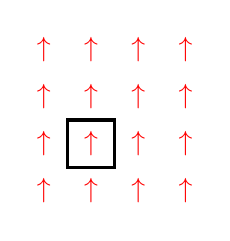
\begin{tikzpicture}[scale=0.6]
  \foreach \x in {0,1,2,3}{\foreach \y in {0,1,2,3}{\node[red] at (\x,\y){$\uparrow$};}}
  \draw[very thick] (0.5,0.5) rectangle (1.5,1.5);
\end{tikzpicture}\\[3pt]
{\footnotesize (a) FM --- cell $1\times1$, $N=1$}
\end{minipage}
\hfill
\begin{minipage}[t]{0.31\textwidth}\centering
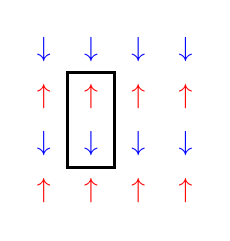
\begin{tikzpicture}[scale=0.6]
  \foreach \x in {0,1,2,3}{\foreach \y in {0,2}{\node[red]  at (\x,\y){$\uparrow$};}}
  \foreach \x in {0,1,2,3}{\foreach \y in {1,3}{\node[blue] at (\x,\y){$\downarrow$};}}
  \draw[very thick] (0.5,0.5) rectangle (1.5,2.5);
\end{tikzpicture}\\[3pt]
{\footnotesize (b) Stripe --- cell $1\times2$, $N=2$}
\end{minipage}
\hfill
\begin{minipage}[t]{0.31\textwidth}\centering
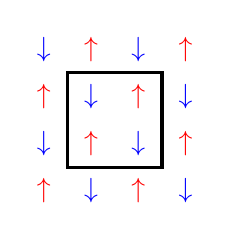
\begin{tikzpicture}[scale=0.6]
  \foreach \x in {0,1,2,3}{\foreach \y in {0,1,2,3}{
    \pgfmathtruncatemacro{\s}{mod(\x+\y,2)}
    \ifnum\s=0 \node[red] at (\x,\y){$\uparrow$};\else\node[blue] at (\x,\y){$\downarrow$};\fi}}
  \draw[very thick] (0.5,0.5) rectangle (2.5,2.5);
\end{tikzpicture}\\[3pt]
{\footnotesize (c) N\'eel --- cell $2\times2$, $N=4$}
\end{minipage}
\caption{The three magnetic orderings of the $J_1$--$J_2$ square lattice used in
the worked example. Red $\uparrow$ and blue $\downarrow$ denote the two collinear
spin directions; nearest neighbours (class \emph{nn}) lie along the axes,
next-nearest neighbours (class \emph{nnn}) along the diagonals. The heavy box
marks the minimal magnetic supercell, containing $N=1$, $2$, and $4$ magnetic
ions respectively.}
\label{fig:orderings}
\end{figure}

A point used repeatedly below: the left-hand side
$\varepsilon_k=E_k^{\mathrm{tot}}/N_k^{\mathrm{mag}}$ is \emph{intensive} and so
takes the same value whether an ordering is represented in its minimal cell or in
a larger one; only the extensive coefficients $C_{ab,k}$ change. The
$\varepsilon$ column is therefore identical in all three matrices that follow.

\subsection{What is correct: a common supercell}
When every ordering is represented in the \emph{same} $2\times2$ cell ($N=4$
throughout), the design matrix is
\begin{equation*}
\begin{array}{l|c|ccc|c}
\text{ordering} & N_k & E_0 & C_{\mathrm{nn}} & C_{\mathrm{nnn}} & \varepsilon~[\mathrm{eV/ion}]\\\hline
\text{FM}     & 4 & 1 & -8 & -8 & -0.012\\
\text{Stripe} & 4 & 1 &  0 & +8 & -0.008\\
\text{N\'eel} & 4 & 1 & +8 & -8 & +0.028
\end{array}
\end{equation*}
Solving $Hx=\boldsymbol\varepsilon$ gives $E_0=0$, $J_{\mathrm{nn}}=+2.5$,
$J_{\mathrm{nnn}}=-1.0$~meV, i.e.\ exactly
$J^{\mathrm{phys}}/N^{\mathrm{mag}}=J^{\mathrm{phys}}/4$. This is the regime the
mapper is built for: every row carries the same factor $N=4$, which factors out
of the solve, and the couplings are recovered up to the common magnetic-ion count
(Sec.~\ref{sec:consistency}).

\subsection{What we would expect for mixed sizes: the intensive/extensive
mismatch}
Suppose instead each ordering is supplied in its minimal cell and---%
hypothetically---the coefficients $C_{ab,k}$ are still computed faithfully for
each cell. Being extensive, they scale with $N_k$ ($C\propto N$): the FM row
shrinks by a factor $4$ and the Stripe row by $2$ relative to the common-cell
values, while the (intensive) $\varepsilon$ column is unchanged:
\begin{equation*}
\begin{array}{l|c|ccc|c}
\text{ordering} & N_k & E_0 & C_{\mathrm{nn}} & C_{\mathrm{nnn}} & \varepsilon~[\mathrm{eV/ion}]\\\hline
\text{FM}     & 1 & 1 & -2 & -2 & -0.012\\
\text{Stripe} & 2 & 1 &  0 & +4 & -0.008\\
\text{N\'eel} & 4 & 1 & +8 & -8 & +0.028
\end{array}
\end{equation*}
Each coupling row now carries a \emph{different} factor $n_k=N_k$. No single
$(E_0,\{J_{ab}\})$ can satisfy rows that demand $J^{\mathrm{phys}}/1$,
$J^{\mathrm{phys}}/2$, and $J^{\mathrm{phys}}/4$ at once. The $3\times3$ system is
nevertheless non-singular, so the solve returns a meaningless blend:
$E_0=-5.8$~meV, $J_{\mathrm{nn}}=+3.67$, $J_{\mathrm{nnn}}=-0.56$~meV---unrelated
to the physical $(+10,-4)$ or to any clean per-ion value. This is precisely the
failure anticipated by Sec.~\ref{sec:consistency}: intensive left-hand side,
extensive right-hand side.

\subsection{What actually happens: the unique-site map is fit to the first
ordering only}
The mapper never reaches the matrix of the previous subsection, because the
entire column scheme is derived from a \emph{single} structure. The unique-site
map is built once, from \code{ordered\_structures[0]} (\code{heisenberg.py:91}),
under the implicit assumption that every ordering shares the same site indexing.
After the energy sort (Sec.~\ref{sec:ingestion}) the lowest-energy ordering sits
first; here that is the FM state in its $1\times1$ cell, so
\begin{equation*}
  \texttt{unique\_site\_ids} = \{(0,)\!:\,0\},
\end{equation*}
which knows only site index $0$. In the row loop each site index is mapped
through this dict (\code{heisenberg.py:285--288} for $i$, \code{:302--305} for
$j$); any index $\ge 1$ is \emph{not found}, its label becomes \code{None}, the
resulting column name (e.g.\ \code{"0-None-nn"}) is absent from the matrix, and
the bond is silently skipped (\code{heisenberg.py:318--321}).
Table~\ref{tab:dropped} records the consequence for each ordering.

\begin{table}[h]
\centering
\caption{Effect of \code{unique\_site\_ids}$=\{(0,)\!:0\}$, built from the FM
$1\times1$ cell, on the larger orderings. Bonds touching any unrecognised site
index are dropped.}
\label{tab:dropped}
\begin{tabularx}{\textwidth}{@{}l l c l X@{}}
\toprule
Ordering (cell) & Site indices & Recognised & Dropped & Surviving bonds \\
\midrule
FM ($1\times1$)     & $\{0\}$       & $0$ & ---       & all (nn and nnn) \\
Stripe ($1\times2$) & $\{0,1\}$     & $0$ & $1$       & only $0$--$0$ image nn \\
N\'eel ($2\times2$) & $\{0,1,2,3\}$ & $0$ & $1,2,3$   & none \\
\bottomrule
\end{tabularx}
\end{table}

The surviving coefficients give
\begin{equation*}
\begin{array}{l|c|ccc|c}
\text{ordering} & N_k & E_0 & C_{\mathrm{nn}} & C_{\mathrm{nnn}} & \varepsilon~[\mathrm{eV/ion}]\\\hline
\text{FM}     & 1 & 1 & -2 & -2 & -0.012\\
\text{Stripe} & 2 & 1 & -1 &  0 & -0.008\\
\text{N\'eel} & 4 & 1 &  0 &  0 & +0.028
\end{array}
\end{equation*}
Only the FM row (a single site, index $0$, mapping cleanly) is correct. The
Stripe row keeps just the site-$0$-to-site-$0$ periodic-image nn bonds (both
spins up, contributing $-1$ after the factor of $\tfrac12$) and loses every bond
to site $1$; the N\'eel row loses \emph{all} of its bonds, because site $0$'s
neighbours are sites $1$, $2$, $3$ exclusively. Solving yields $E_0=+28$~meV,
$J_{\mathrm{nn}}=+36$, $J_{\mathrm{nnn}}=-16$~meV---pure nonsense, and produced
with no error and no warning. Table~\ref{tab:threecases} collects the three
outcomes.

\begin{table}[h]
\centering
\caption{Couplings returned in the three scenarios. Physical truth:
$J_{\mathrm{nn}}=+10$, $J_{\mathrm{nnn}}=-4$~meV.}
\label{tab:threecases}
\begin{tabularx}{\textwidth}{@{}X c c c@{}}
\toprule
Scenario & $E_0$ & $J_{\mathrm{nn}}$ [meV] & $J_{\mathrm{nnn}}$ [meV] \\
\midrule
Common $2\times2$ cell (correct)                       & $0$        & $+2.5$  & $-1.0$  \\
Mixed minimal cells, faithful coefficients (hypothetical) & $-5.8$~meV & $+3.67$ & $-0.56$ \\
Mixed minimal cells, actual code                        & $+28$~meV  & $+36$   & $-16$   \\
\bottomrule
\end{tabularx}
\end{table}

\paragraph{Two distinct failure modes.} The example separates two faults that the
single-parent-cell workflow hides. (1)~The \emph{normalisation asymmetry} of
Sec.~\ref{sec:consistency}---intensive $\varepsilon$ against extensive
$C_{ab,k}$---makes a mixed-size fit ill-posed even with perfectly computed
coefficients. (2)~The \emph{unique-site map}, built from
\code{ordered\_structures[0]} alone, hard-codes one common site indexing; mixed
sizes drop every bond involving an index beyond the first structure's atom count,
so the code does not even degrade gracefully to mode~(1)---it produces a matrix
dominated by dropped terms. Both faults are inert when all orderings share a
single supercell, the standard enumeration workflow, which is why the restriction
of Sec.~\ref{sec:consistency} is the operative one in practice.

\section{Conclusion}

We have traced the energy through pymatgen's \code{HeisenbergMapper} from total
DFT energies to the serialised \code{HeisenbergModel}. The mapper applies exactly
one normalisation---division by the number of magnetic ions---so it operates
entirely in eV per magnetic ion internally and reports couplings in meV per
magnetic ion, despite the ``meV/atom'' labelling in the source. The fitted
couplings coincide with the physical exchange constants (up to the common
magnetic-ion count) only when every ordering shares the same absolute supercell
size; this condition holds for the standard single-parent-cell magnetic-orderings
workflow but fails when supercells of different sizes are mixed. The worked
example of Sec.~\ref{sec:example} makes this concrete and exposes two independent
failure modes for mixed sizes: the intensive/extensive normalisation asymmetry of
Sec.~\ref{sec:consistency}, which makes the fit ill-posed even with faithful
coefficients, and a more basic one---the unique-site map is constructed from
\code{ordered\_structures[0]} alone, so bonds involving site indices beyond the
first structure's atom count are silently dropped, yielding a corrupted matrix
with no error raised. We additionally noted a pandas-version-dependent defect in
the singularity guard of the design-matrix routine (Sec.~\ref{sec:design}), which
affects only the degenerate all-zero-column case.

\end{document}
